%%% You need to use XeLaTeX to compile this project
\documentclass[12pt,a4paper,oneside]{book}
\usepackage{thesis-ict}

%%% Packages
\usepackage{enumitem}
\usepackage{listings}
\usepackage[table]{xcolor}
\usepackage{minted}
\usepackage{multirow}
\usepackage{booktabs}
\usepackage[sort,nobreak]{cite}
\usepackage[nameinlink]{cleveref} % https://tex.stackexchange.com/a/54274
\usepackage[dvipdfmx]{graphicx}
\usepackage{import}
\usepackage[labelformat=simple,labelfont=bf]{subcaption} % Format simple removes ()
\usepackage[nottoc]{tocbibind} % https://tex.stackexchange.com/a/8459
\usepackage{setspace}\doublespacing

%%% Options
\crefname{chapter}{Chapter}{Chapters}
\crefname{section}{Section}{Sections}
\crefname{equation}{Equation}{Equations}
\crefname{figure}{Figure}{Figures}
\crefname{table}{Table}{Tables}
\crefname{appendix}{Appendix}{Appendices}
\renewcommand{\figurename}{\textbf{Figure}}
\renewcommand{\tablename}{\textbf{Table}}
\renewcommand{\thetable}{\arabic{chapter}.\arabic{table}}
\renewcommand{\thefigure}{\arabic{chapter}.\arabic{figure}}
\renewcommand{\thesubfigure}{(\alph{subfigure})} % Add the () here not when loading subcaption 
\captionsetup[figure]{labelsep=colon,labelfont=bf}
\captionsetup[table]{labelsep=colon,labelfont=bf}
\definecolor{gray90}{gray}{0.9} % https://texblog.org/2011/09/02/coloring-every-alternate-table-row/
\lstset{basicstyle=\ttfamily}
\renewcommand\bibname{References}
\setlist[itemize]{topsep=10pt,partopsep=4pt,parsep=2pt,itemsep=2pt,listparindent=\parindent{}}
\setlist[enumerate]{topsep=10pt,partopsep=4pt,parsep=2pt,itemsep=2pt,listparindent=\parindent{}}

%%% Thesis information; change accordingly (title, your name, advisor(s) and date)
\parindent 1em
\title{Title}
\author{Alice Suzukakedai}
\advisorA{Bob Ookayama}
\advisorAjobtitle{Professor}
% In case you have another advisor use the following:
% \advisorB{Carol Ishikawadai}
% \advisorBjobtitle{Associate Professor}
\date{August 2022}

\begin{document}

\frontmatter
\maketitle
\mbox{}
\thispagestyle{empty}
\newpage

\chapter*{Abstract}
\setcounter{page}{1}

Write the abstract of the thesis.
Please aim at writing around 400 words.
You'll be submitting the abstract to the school later.          % Sample
% \chapter*{Abstract}
\setcounter{page}{1}

Write the abstract of the thesis.
Please aim at writing around 400 words.
You'll be submitting the abstract to the school later.
\tableofcontents
\listoffigures
\listoftables
\chapter*{Publications}\label{ch:publication}
\addcontentsline{toc}{chapter}{Publications}
% \addcontentsline{toc}{chapter}{\numberline{}Publications} % https://tex.stackexchange.com/a/25799

If you have none, you can omit this chapter by commenting out the according \texttt{\textbackslash{}input\{\}} from \texttt{main.tex}.      % Sample
% \chapter*{Publications}\label{ch:publication}

\section*{Conference Papers}

\chapter*{Acknowledgments}
\addcontentsline{toc}{chapter}{Acknowledgments}
% \addcontentsline{toc}{chapter}{\numberline{}Acknowledgments} % https://tex.stackexchange.com/a/25799

You can acknowledge whomever and whatever helped you write the thesis.  % Sample
% \chapter*{Acknowledgments}
\addcontentsline{toc}{chapter}{Acknowledgments}
% \addcontentsline{toc}{chapter}{\numberline{}Acknowledgments} % https://tex.stackexchange.com/a/25799

You can acknowledge whomever and whatever helped you write the thesis.


\mainmatter
\chapter{Introduction}\label{ch:introduction}

Write the introduction of the thesis.
Make sure you assume a reader who is not familiar with the research area.

Throughout the paper you should cite proper references\cite{bar:great2020coolname}.\footnote{I think you would cite at least 30 papers.}
List all the references in \texttt{main.bib} file and cite them using the \texttt{{\textbackslash}cite\{\}} command.
You can also cite multiple papers at once\cite{garply:happy2021anothercoolname,bar:great2020coolname}.
The \texttt{cite} package with \texttt{sort} option (which is enabled by default) allows sorting the references as in [1,~2] and not [2,~1], please compare with the previous sentence\cite{bar:great2020coolname,garply:happy2021anothercoolname}.
You do not need to manually add a space (using {\textasciitilde}) before the \texttt{{\textbackslash}cite\{\}} command because \texttt{cite} package takes care of it too.

You might want to decorate (using \textit{italic}, \textbf{bold} and \underline{underline}) certain words or sentences to emphasize important things.
In general \textit{italic} is the first choice in English.
One last thing, I believe writing one sentence in one line (in \LaTeX source code) is the best practice.    % Sample
% \chapter{Introduction}\label{ch:introduction}


\chapter{Background}\label{ch:background}

\section{Research Background: Part~1}\label{sec:background1}

Discuss the background (e.g., basic knowledge, related studies etc) of your research project.
As in \cref{ch:introduction}\footnote{Always use cleverref's {\textbackslash}cref\{\} command to reference sections, figures and tables. It will automatically use the format defined in main.tex so you do not need to deal with it on your own.} you need to assume your readers are not familiar with your research. Be kind.
Yet, don't be too talkative, be concise and to the point.

Also do not forget to change the section names inside {\textbackslash}section\{\}, for instance ``Research Background: Part~1'' is just an example.

\section{Research Background: Part~2}\label{sec:background2}

You may use ordered (or numbered) lists to better organize your thesis:
\begin{enumerate}
  \item First item;
  \item second item; and
  \item the third.
\end{enumerate}      % Sample
% \chapter{Background}\label{ch:background}

\section{Research Background: Part~1}\label{sec:background1}

Discuss the background (e.g., basic knowledge, related studies etc) of your research project.
As in \cref{ch:introduction}\footnote{Always use cleverref's {\textbackslash}cref\{\} command to reference sections, figures and tables. It will automatically use the format defined in main.tex so you do not need to deal with it on your own.} you need to assume your readers are not familiar with your research. Be kind.
Yet, don't be too talkative, be concise and to the point.

Also do not forget to change the section names inside {\textbackslash}section\{\}, for instance ``Research Background: Part~1'' is just an example.

\section{Research Background: Part~2}\label{sec:background2}

You may use ordered (or numbered) lists to better organize your thesis:
\begin{enumerate}
  \item First item;
  \item second item; and
  \item the third.
\end{enumerate}
\chapter{Motivation}\label{ch:motivation}

In addition to the numbered list introduced in \cref{sec:background2}, you can also use the unordered (or bullet) list as below.
For instance you may organize this chapter with the following flow:
\begin{itemize}
  \item Introduce the weaknesses and remaining problems to be solved of the related studies introduced in \cref{ch:background}.
  \item Discuss the key observation/insight/hypothesis which led to the proposal of your thesis that aims at solving one of the problems explained above.
  \item Demonstrate the potential of your idea for instance through an initial experiment with ideal conditions (e.g., ideal parameters such as zero latency or infinite bandwidth).
  \item Using the results above motivate your study with quantitative evidence.
\end{itemize}
It might be better to explain the background and discuss your motivation in a single chapter.
In that case you may combine this chapter with \cref{ch:background}.      % Sample
% \chapter{Motivation}\label{ch:motivation}

In addition to the numbered list introduced in \cref{sec:background2}, you can also use the unordered (or bullet) list as below.
For instance you may organize this chapter with the following flow:
\begin{itemize}
  \item Introduce the weaknesses and remaining problems to be solved of the related studies introduced in \cref{ch:background}.
  \item Discuss the key observation/insight/hypothesis which led to the proposal of your thesis that aims at solving one of the problems explained above.
  \item Demonstrate the potential of your idea for instance through an initial experiment with ideal conditions (e.g., ideal parameters such as zero latency or infinite bandwidth).
  \item Using the results above motivate your study with quantitative evidence.
\end{itemize}
It might be better to explain the background and discuss your motivation in a single chapter.
In that case you may combine this chapter with \cref{ch:background}.
\chapter{Proposed System}\label{ch:proposedsytem}

Explain your proposed system/mechanism/technique.
Figures are effective so better use them accordingly.
Vector images are more beautiful than bitmaps so it is recommended to use pdf files.\footnote{Same can be said for graphs which we will see in \cref{sec:results}.}
One caveat is that you do not want to have blank spaces surrounding your pdf file.
If you have some, you can delete them by using commands such as:

\begin{minted}[bgcolor=gray90]{bash}
% pdfcrop --margins 0 input.pdf output.pdf
\end{minted}

% Code below becomes an error for xelatex (not for platex)
% \begin{lstlisting}[language=bash,escapeinside={(*}{*)}]
% (*\colorbox{gray90}{\% pdfcrop --margins 0 input.pdf output.pdf}*)
% \end{lstlisting}

\begin{figure}[ht]
  \centering
  
\includegraphics[width=0.5\textwidth]{examples/figures/square}
  \caption{A square.}\label{fig:square}
\end{figure}

Always refer to the figure in your body.
\cref{fig:square} is a square.

\begin{figure}[ht]
  \centering
  \begin{subfigure}[t]{0.45\textwidth}
  \centering
    
\includegraphics[width=0.8\linewidth]{examples/figures/square}
    \caption{A square.}\label{subfig:square}
  \end{subfigure}
  \quad
  \begin{subfigure}[t]{0.45\textwidth}
  \centering
    
\includegraphics[width=0.8\linewidth]{examples/figures/circle}
    \caption{A circle.}\label{subfig:circle}
  \end{subfigure}
  \caption{A square and a circle.}\label{fig:square-circle}
\end{figure}

\cref{fig:square-circle} shows a square and a circle, while \cref{subfig:circle} represents only the circle.  % Sample
% \chapter{Proposed System}\label{ch:proposedsytem}

Explain your proposed system/mechanism/technique.
Figures are effective so better use them accordingly.
Vector images are more beautiful than bitmaps so it is recommended to use pdf files.\footnote{Same can be said for graphs which we will see in \cref{sec:results}.}
One caveat is that you do not want to have blank spaces surrounding your pdf file.
If you have some, you can delete them by using commands such as:

\begin{minted}[bgcolor=gray90]{bash}
% pdfcrop --margins 0 input.pdf output.pdf
\end{minted}

% Code below becomes an error for xelatex (not for platex)
% \begin{lstlisting}[language=bash,escapeinside={(*}{*)}]
% (*\colorbox{gray90}{\% pdfcrop --margins 0 input.pdf output.pdf}*)
% \end{lstlisting}

\begin{figure}[ht]
  \centering
  
\includegraphics[width=0.5\textwidth]{examples/figures/square}
  \caption{A square.}\label{fig:square}
\end{figure}

Always refer to the figure in your body.
\cref{fig:square} is a square.

\begin{figure}[ht]
  \centering
  \begin{subfigure}[t]{0.45\textwidth}
  \centering
    
\includegraphics[width=0.8\linewidth]{examples/figures/square}
    \caption{A square.}\label{subfig:square}
  \end{subfigure}
  \quad
  \begin{subfigure}[t]{0.45\textwidth}
  \centering
    
\includegraphics[width=0.8\linewidth]{examples/figures/circle}
    \caption{A circle.}\label{subfig:circle}
  \end{subfigure}
  \caption{A square and a circle.}\label{fig:square-circle}
\end{figure}

\cref{fig:square-circle} shows a square and a circle, while \cref{subfig:circle} represents only the circle.
\chapter{Evaluation}\label{ch:evaluation}

\section{Evaluation Methodology}\label{sec:methodology}

For instance you can explain the hardware and software you used for your evaluation.
Explain all the details necessary for the readers to be able to reproduce your experiments.
Tables can be effective so use them accordingly.

\begin{table}[ht]
  \centering
  \caption{A table with lots of numbers.}{
  \rowcolors{3}{gray90}{}
  \resizebox{0.95\textwidth}{!}{
    {\renewcommand{\arraystretch}{1.3}
    \begin{tabular}{c>{\hspace{1pc}}c c c>{\hspace{1pc}}c c c} % https://tex.stackexchange.com/a/31704
      \toprule
      \multirow{2}{*}{Techniques we compare} & \multicolumn{3}{c}{Results (absolute values)} & \multicolumn{3}{c}{Results (relative to baseline)} \\
             & Area($mm^2$) & Delay($ns$) & Power($m W$) & Area(\%)  & Delay(\%) & Power(\%) \\
      \midrule
            Baseline &   347,329.19 &       1.62 &       15.84 &       --- &      --- &      --- \\
Proposed technique 1 &   412,263.87 &       1.65 &       16.17 &     18.69 &     1.85 &     2.12 \\
Proposed technique 2 &   370,972.35 &       2.42 &       17.95 &      6.80 &    49.38 &    11.00 \\
Proposed technique 3 &   356,694.82 &       1.98 &       16.00 &      2.69 &    22.22 &     1.06 \\
      \bottomrule
    \end{tabular}}\label{tab:example}
  }
}
\end{table}

\cref{tab:example} shows a lot of numbers.
Tables look better without vertical lines (some of you might have seen the linter message: ``Vertical rules in tables are ugly.'').
Also the odd rows are shaded in gray.
It greatly enhances the readability (especially with tables with many rows/columns) so is recommended to use it.

\section{Evaluation Results}\label{sec:results}

Quantitatively evaluate your proposed system/technique and discuss them.
Graphs are effective so use them accordingly.

\begin{figure}[ht]
  \centering
  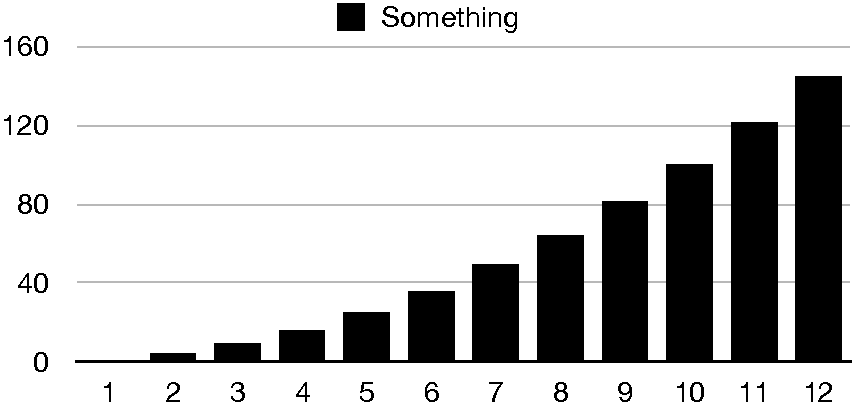
\includegraphics[width=0.9\textwidth]{examples/graphs/something}
  \caption{Trend of something.}\label{fig:something}
\end{figure}

If you look at \cref{fig:something}, we can see that the value of something is exponentially growing.
We present the detailed data of the evaluation results in \cref{ch:appendix2}.      % Sample
% \chapter{Evaluation}\label{ch:evaluation}

\section{Evaluation Methodology}\label{sec:methodology}

For instance you can explain the hardware and software you used for your evaluation.
Explain all the details necessary for the readers to be able to reproduce your experiments.
Tables can be effective so use them accordingly.

\begin{table}[ht]
  \centering
  \caption{A table with lots of numbers.}{
  \rowcolors{3}{gray90}{}
  \resizebox{0.95\textwidth}{!}{
    {\renewcommand{\arraystretch}{1.3}
    \begin{tabular}{c>{\hspace{1pc}}c c c>{\hspace{1pc}}c c c} % https://tex.stackexchange.com/a/31704
      \toprule
      \multirow{2}{*}{Techniques we compare} & \multicolumn{3}{c}{Results (absolute values)} & \multicolumn{3}{c}{Results (relative to baseline)} \\
             & Area($mm^2$) & Delay($ns$) & Power($m W$) & Area(\%)  & Delay(\%) & Power(\%) \\
      \midrule
            Baseline &   347,329.19 &       1.62 &       15.84 &       --- &      --- &      --- \\
Proposed technique 1 &   412,263.87 &       1.65 &       16.17 &     18.69 &     1.85 &     2.12 \\
Proposed technique 2 &   370,972.35 &       2.42 &       17.95 &      6.80 &    49.38 &    11.00 \\
Proposed technique 3 &   356,694.82 &       1.98 &       16.00 &      2.69 &    22.22 &     1.06 \\
      \bottomrule
    \end{tabular}}\label{tab:example}
  }
}
\end{table}

\cref{tab:example} shows a lot of numbers.
Tables look better without vertical lines (some of you might have seen the linter message: ``Vertical rules in tables are ugly.'').
Also the odd rows are shaded in gray.
It greatly enhances the readability (especially with tables with many rows/columns) so is recommended to use it.

\section{Evaluation Results}\label{sec:results}

Quantitatively evaluate your proposed system/technique and discuss them.
Graphs are effective so use them accordingly.

\begin{figure}[ht]
  \centering
  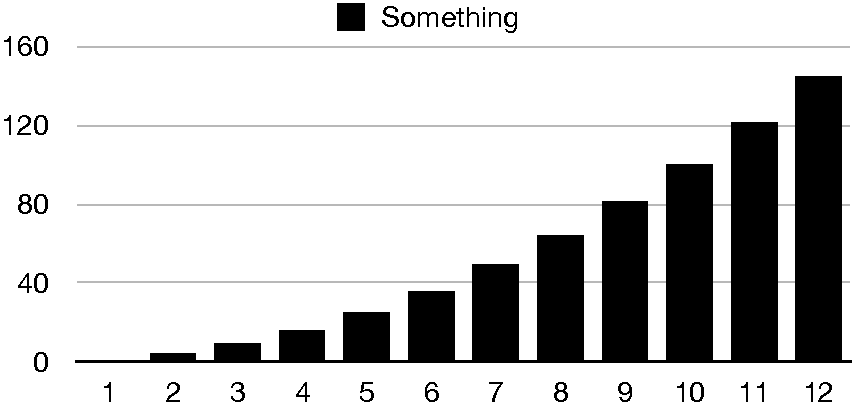
\includegraphics[width=0.9\textwidth]{examples/graphs/something}
  \caption{Trend of something.}\label{fig:something}
\end{figure}

If you look at \cref{fig:something}, we can see that the value of something is exponentially growing.
We present the detailed data of the evaluation results in \cref{ch:appendix2}.
\chapter{Related Work}\label{ch:relatedwork}

Here you can introduce related work which are not as important as the ones you discussed in \cref{ch:background} but would help put your work into context.
Therefore, it is important to explain the important differences between your work and theirs.

Also beware it is ``Related Work'' and not ``Related Works''.     % Sample
% \chapter{Related Work}\label{ch:relatedwork}

Here you can introduce related work which are not as important as the ones you discussed in \cref{ch:background} but would help put your work into context.
Therefore, it is important to explain the important differences between your work and theirs.

Also beware it is ``Related Work'' and not ``Related Works''.
\chapter{Conclusion}\label{ch:conclusion}

Briefly recap your study.
What was the problem you solved, what were the key observations/ideas that led to your proposal, what were the results etc.
You may briefly touch upon how you can extend your study in the future.      % Sample
% \chapter{Conclusion}\label{ch:conclusion}

Briefly recap your study.
What was the problem you solved, what were the key observations/ideas that led to your proposal, what were the results etc.
You may briefly touch upon how you can extend your study in the future.
\appendix

\chapter{Proof of Lemma~1}\label{ch:appendix1}

\chapter{Detailed Data of \cref{sec:results}}\label{ch:appendix2}          % Sample
% \appendix

\chapter{Proof of Lemma~1}\label{ch:appendix1}

\chapter{Detailed Data of \cref{sec:results}}\label{ch:appendix2}

% \backmatter
% \include{acknowledgement}
% \newcommand{\BIBdecl}{\setlength{\itemsep}{0.27 em}}
\bibliographystyle{unsrt}
\bibliography{examples/main}       % Sample
% \bibliography{main}

\end{document}